\chapter{A Gentle Introduction to GObject}
\label{oop-gobject}

In the previous chapter we have learned how to write semi-object-oriented code in C. This is how the classes in GLib core are written. GObject goes several steps further into Object-Oriented Programming, with inheritance, interfaces, virtual functions, etc. GObject also simplifies the event-driven programming paradigm, with signals and properties.

It is recommended to create your own GObject classes for writing a GLib/GTK+ application. Unfortunately the code is a little verbose, because the C language is not object-oriented. Boilerplate code is needed for some features, but don't be afraid, there are tools and scripts to generate the boilerplate.

However this chapter takes a step back from the previous chapter, it is just a small introduction to GObject; it will explain the essential things to know how to \emph{use} an existing GObject class (like all GTK+ widgets and classes in GIO). It will not explain how to \emph{create} your own GObject classes, because it is already well covered in the GObject reference manual, and the goal of this book is not to duplicate the whole content of the reference manuals, the goal is more to serve as a getting started guide.

So for more in-depth information on GObject and to know how to create sub-classes, the GObject reference documentation contains introductory chapters: ``\emph{Concepts}'' and ``\emph{Tutorial}'', available at:

\url{https://developer.gnome.org/gobject/stable/}

To explain certain concepts, some examples are taken from GTK+ or GIO. When reading this chapter, you are encouraged to open in parallel Devhelp, to look at the API reference and see for yourself how a GObject-based library is documented. The goal is that you become autonomous and be able to learn any new GObject class, be it in GIO, GTK+ or any other library.

\section{Inheritance}
\label{oop-gobject-inheritance}

An important concept of OOP is inheritance. A class can be a sub-class of a parent class. The sub-class inherits the features of the parent class, extending or overriding its behavior.

The GObject library provides the \lstinline{GObject} base class. Every class in GIO and GTK+ inherit --- directly or indirectly --- from the \lstinline{GObject} base class. When looking at a GObject-based class, the documentation (if written with GTK-Doc) always contains an \emph{Object Hierarchy}. For instance, the \lstinline{GtkApplication} has the following object hierarchy:

\begin{verbatim}
GObject
└── GApplication
    └── GtkApplication
\end{verbatim}

It means that when you create a \lstinline{GtkApplication} object, you also have access to the functions, signals and properties of \lstinline{GApplication} (implemented in GIO) and \lstinline{GObject}. Of course, the \lstinline{g_application_*} functions take as first argument a variable of type ``\lstinline{GApplication *}'', not ``\lstinline{GtkApplication *}''. To cast the variable to the good type, the recommended way is to use the \lstinline{G_APPLICATION()} macro. For example:

\begin{lstlisting}
GtkApplication *app;

g_application_mark_busy (G_APPLICATION (app));
\end{lstlisting}

\section{GObject Macros}

Each GObject class provides a set of standard macros. The \lstinline{G_APPLICATION()} macro as demonstrated in the previous section is one of the standard macros provided by the \lstinline{GApplication} class.

Not all the standard GObject macros will be explained here, just the macros useful for \emph{using} a GObject in a basic way. The other macros are more advanced and are usually useful only when sub-classing a GObject class, when creating a property or a signal, or when overriding a virtual function.

Each GObject class defines a macro of the form \lstinline{NAMESPACE_CLASSNAME(object)}, which casts the variable to the type ``\lstinline{NamespaceClassname *}'' and checks at runtime if the variable correctly contains a \lstinline{NamespaceClassname} object or a sub-class of it. If the variable is \lstinline{NULL} or contains an incompatible object, the macro prints a critical warning message to the console and returns NULL.

A standard cast works too, but is most of the time not recommended because there are no runtime checks:
\begin{lstlisting}
GtkApplication *app;

/* Not recommended */
g_application_mark_busy ((GApplication *) app);
\end{lstlisting}

Another macro useful when using a GObject is \lstinline{NAMESPACE_IS_CLASSNAME(object)}, which returns \lstinline{TRUE} if the variable is a \lstinline{NamespaceClassname} object or a sub-class of it.

%TODO show an example of a function checking its arguments with g_return?

\section{Interfaces}

With GObject it is possible to create interfaces. An interface is just an API, it doesn't contain the implementation. A GObject class can implement one or several interfaces. If a GObject class is documented with GTK-Doc, the documentation will contain a section \emph{Implemented Interfaces}.

For example GTK+ contains the \lstinline{GtkOrientable} interface that is implemented by many widgets and permits to set the orientation: horizontal or vertical.

The two macros explained in the previous section work for interfaces too. An example with \lstinline{GtkGrid}:
\begin{lstlisting}
GtkWidget *vgrid;

vgrid = gtk_grid_new ();
gtk_orientable_set_orientation (GTK_ORIENTABLE (vgrid),
                                GTK_ORIENTATION_VERTICAL);
\end{lstlisting}

So when you search a certain feature in the API for a certain GObject class, the feature can be located at three different places:
\begin{itemize}
  \item In the GObject class itself;
  \item In one of the parent classes in the \emph{Object Hierarchy};
  \item Or in one of the \emph{Implemented Interfaces}.
\end{itemize}

\section{Reference Counting}

The memory management of GObject classes rely on \emph{reference counting}. A GObject class has a counter:
\begin{itemize}
  \item When the object is created the counter is equal to one;
  \item \lstinline{g_object_ref()} increments the counter;
  \item \lstinline{g_object_unref()} decrements the counter;
  \item If the counter reaches zero, the object is freed.
\end{itemize}

It permits to store the GObject at several places without the need to coordinate when to free the object.

\subsection{Avoiding Reference Cycles with Weak References}

If object A references object B and object B references object A, there is a reference cycle and the two objects will never be freed. To avoid that problem, there is the concept of ``weak'' references. When calling \lstinline{g_object_ref()}, it's a ``strong'' reference. So in one direction there is a strong reference, and in the other direction there must be a weak reference (or no references at all).

\begin{figure}
  \begin{center}
    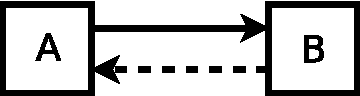
\includegraphics[scale=0.75]{images/weak-ref.pdf}
    \caption{Using a weak reference to break the reference cycle between A and B.}
    \label{oop-gobject-weak-ref-schema}
  \end{center}
\end{figure}

In Figure~\ref{oop-gobject-weak-ref-schema} we can see that object A has a strong reference to object B, and object B has a weak reference to object A.

A weak reference can be created with \lstinline{g_object_add_weak_pointer()} or \lstinline{g_object_weak_ref()}. As with strong references, it is important to release the reference when no longer needed, usually in the class destructor. A weak reference must be removed with \lstinline{g_object_remove_weak_pointer()} or \lstinline{g_object_weak_unref()}. So in Figure~\ref{oop-gobject-weak-ref-schema}, the destructor of class B must remove the weak reference if it is not already done.

\subsection{Floating References}

When a GObject class inherits from \lstinline{GInitiallyUnowned} (which is the case of \lstinline{GtkWidget}), the object initially has a \emph{floating} reference. \lstinline{g_object_ref_sink()} must be called to convert that floating reference into a normal, strong reference.

When a GObject inherits from \lstinline{GInitiallyUnowned}, it means that that GObject is meant to be included in some kind of container. The container then assumes ownership of the floating reference, calling \lstinline{g_object_ref_sink()}. It permits to simplify the code, to remove the need to call \lstinline{g_object_unref()} after including the object into the container.

The Listing~\ref{oop-gobject-mem-management-normal} p.~\pageref{oop-gobject-mem-management-normal} shows how memory management is handled with a normal GObject. Compare this to the Listing~\ref{oop-gobject-mem-management-floating}, which shows how memory management is handled with a GObject deriving from \lstinline{GInitiallyUnowned}. The difference is that \lstinline{g_object_unref()} is not called in the latter Listing, so it shortens the code.

\begin{lstlisting}[float=p, caption={Memory management of normal GObjects.}, label=oop-gobject-mem-management-normal]
/* Normal GObject */

a_normal_gobject = normal_gobject_new ();
/* a_normal_gobject has now a reference count of 1. */

container_add (container, a_normal_gobject);
/* a_normal_gobject has now a reference count of 2. */

/* We no longer need a_normal_gobject, so we unref it. */
g_object_unref (a_normal_gobject);
/* a_normal_gobject has now a reference count of 1. */
\end{lstlisting}

\begin{lstlisting}[float=p, caption={Memory management of GObjects deriving from \lstinline{GInitiallyUnowned}.}, label=oop-gobject-mem-management-floating]
/* GInitiallyUnowned object, e.g. a GtkWidget */

widget = gtk_entry_new ();
/* widget has now just a floating reference. */

gtk_container_add (container, widget);
/* The container has called g_object_ref_sink(), taking
 * ownership of the floating reference. The code is
 * simplified because we must not call g_object_unref().
 */
\end{lstlisting}

So, it's important to know whether a GObject inherits from \lstinline{GInitiallyUnowned} or not. For that you need to look at the \emph{Object Hierarchy}, for example \lstinline{GtkEntry} has the following hierarchy:

\begin{verbatim}
GObject
└── GInitiallyUnowned
    └── GtkWidget
        └── GtkEntry
\end{verbatim}

\section{Signals and Properties}
\label{oop-gobject-signals-and-properties}

A GObject class can emit signals. With the GLib main event loop (previously explained in section~\ref{glib-main-event-loop} p.~\pageref{glib-main-event-loop}), this is the foundation for event-driven programming. An example of a signal is when the user clicks on a button. The application connects a callback function to the signal to perform the desired action when the event occurs.

Another concept of GObject are \emph{properties}, which is related to signals. A property is basically an instance variable surmounted with a \lstinline{"notify"} signal that is emitted when its value changes. A good example of a property is the state of a check button, i.e. a boolean value describing whether the button is currently checked or not. When the state changes, the \lstinline{"notify"} signal is sent.

To create your own signals or properties, a GObject sub-class must be created. As explained in the introduction of this chapter, this is beyond the scope of this book, but you should be aware that creating your own signals or properties is of course possible, and recommended. In fact, creating a GObject signal or property is a nice way to implement the Observer design pattern \cite{design-patterns-book}; that is, one or several objects \emph{observing} state changes of another object, by connecting function callbacks. The object \emph{emitting} the signal is not aware of which objects \emph{receive} the signal. GObject just keeps track of the list of callbacks to call. So adding a signal permits to decouple classes.

\subsection{Connecting a Callback Function to a Signal}

To make things more concrete, if you look at the \lstinline{GtkButton} documentation, you'll see that it provides the \lstinline{"clicked"} signal. To perform the desired action when the signal is emitted, one or more callback function(s) must be connected beforehand.

To connect a callback to a signal, the \lstinline{g_signal_connect()} function can be used, or one of the other \lstinline{g_signal_connect_*()} functions:
\begin{itemize}
  \item \lstinline{g_signal_connect()}
  \item \lstinline{g_signal_connect_after()}
  \item \lstinline{g_signal_connect_swapped()}
  \item \lstinline{g_signal_connect_data()}
  \item \lstinline{g_signal_connect_object()}
  \item And a few more advanced ones.
\end{itemize}

The Listing~\ref{oop-gobject-gtkbutton-clicked} p.~\pageref{oop-gobject-gtkbutton-clicked} shows the prototype of the \lstinline{GtkButton::clicked} signal\footnote{The convention when referring to a GObject signal is ``\lstinline{ClassName::signal-name}''. That's how it is documented with GTK-Doc comments.}.

\begin{lstlisting}[float, caption={The prototype of the \lstinline{GtkButton::clicked} signal.}, label=oop-gobject-gtkbutton-clicked]
void
user_function (GtkButton *button,
               gpointer   user_data);
\end{lstlisting}

When using \lstinline{g_signal_connect()}, the callback function must have the same prototype as the signal prototype. A lot of signals have more arguments, and some signals return a value. If the callback has an incompatible prototype, bad things will happen, there will be random bugs or crashes.

The Listing~\ref{oop-gobject-connect-to-signal} p.~\pageref{oop-gobject-connect-to-signal} shows an example of how to use \lstinline{g_signal_connect()}.

\begin{lstlisting}[float, caption={How to connect to a signal}, label=oop-gobject-connect-to-signal]
static void
button_clicked_cb (GtkButton *button,
                   gpointer   user_data)
{
  MyClass *my_class = MY_CLASS (user_data);

  g_message ("Button clicked!");
}

static void
create_button (MyClass *my_class)
{
  GtkButton *button;

  /* Create the button */
  /* ... */

  /* Connect the callback function */
  g_signal_connect (button,
                    "clicked",
                    G_CALLBACK (button_clicked_cb),
                    my_class);
}
\end{lstlisting}

The \lstinline{G_CALLBACK()} macro is necessary because \lstinline{g_signal_connect()} is generic: it can be used to connect to any signal of any GObject class, so the function pointer needs to be casted.

There are two main conventions to name callback functions:
\begin{itemize}
  \item End the function name with ``\lstinline{cb}'', shortcut for ``callback''. For example: \lstinline{button_clicked_cb()} as in the above code sample.
  \item Start the function name with ``\lstinline{on}''. For example: \lstinline{on_button_clicked()}.
\end{itemize}

With one of those naming conventions --- and with the \lstinline{gpointer user_data} parameter, which is always the last parameter --- it is easy to recognize that a function is a callback.

The C language permits to write a different --- but compatible --- callback function signature, although it is not universally seen as a good thing to do:
\begin{itemize}
  \item One or more of the \emph{last} function argument(s) can be omitted if they are not used. But as explained above the \lstinline{gpointer user_data} argument permits to easily recognize that the function is effectively a callback\footnote{As with natural languages, redundancy permits to better and more quickly understand what we read or listen to.}.
  \item The types of the arguments can be modified to a compatible type: e.g. another class in the inheritance hierarchy, or in the above example, replacing ``\lstinline{gpointer}'' by ``\lstinline{MyClass *}'' (but doing that makes the code a bit less robust because the \lstinline{MY_CLASS()} macro is not called).
\end{itemize}

\subsection{Disconnecting Signal Handlers}

In Listing~\ref{oop-gobject-connect-to-signal}, \lstinline{button_clicked_cb()} is called each time that the \lstinline{button} object emits the \lstinline{"clicked"} signal. If the \lstinline{button} object is still alive after \lstinline{my_class} has been freed, when the signal will be emitted again there will be a little problem… So in the destructor of \lstinline{MyClass}, the signal handler (i.e. the callback) must be disconnected. How to do that?

The \lstinline{g_signal_connect*()} functions actually return an ID of the signal handler, as a \lstinline{gulong} integer always greater than 0 (for successful connections). By storing that ID, it is possible to disconnect that specific signal handler with the \lstinline{g_signal_handler_disconnect()} function.

Sometimes we also want to disconnect the signal handler simply because we are no longer interested by the event.

The Listing~\ref{oop-gobject-disconnect-signal} shows a complete example of how to disconnect a signal handler when its \lstinline{user_data} argument is freed. We come back to an example with a spell checker, because the example with the GTK+ button doesn't fit well the situation\footnote{Most of the time a GTK+ widget doesn't live longer than the container it is added to, and the object listening to the widget signal is usually the container itself. So if the widget dies at the same time as the container, it is not possible for the widget to send a signal while its container has already been destroyed. In that case, there is thus no point in disconnecting the signal in the container destructor, since at that point the widget is already freed; and it's harder for a dead object to send a signal\footnotemark.}.
% GObject is boring so a bit of humor doesn't hurt, a footnote inside a footnote, footception :-)
\footnotetext{When I say that it is harder, it is actually impossible, of course.}

The \lstinline{user_data} callback argument is a \lstinline{MyTextView} instance, with \lstinline{MyTextView} implemented with a semi-OOP style. Since the spell checker object can live longer than the \lstinline{MyTextView} instance, the signal needs to be disconnected in the \lstinline{MyTextView} destructor.

\vspace{0.7cm}
\lstinputlisting[caption={Disconnecting a signal handler when its \lstinline{user_data} argument is freed.}, label=oop-gobject-disconnect-signal]{code/disconnect-signal.c}

There are actually other \lstinline{g_signal_handler*()} functions that permit to disconnect signal handlers:
\begin{itemize}
  \item \lstinline{g_signal_handlers_disconnect_by_data()}
  \item \lstinline{g_signal_handlers_disconnect_by_func()}
  \item \lstinline{g_signal_handlers_disconnect_matched()}
\end{itemize}

It would have been possible to use one of the above functions in Listing~\ref{oop-gobject-disconnect-signal}, and it would have avoided the need to store \lstinline{word_added_to_personal_handler_id}. The basic \lstinline{g_signal_handler_disconnect()} function has been used for learning purposes.

Note also that if \lstinline{MyTextView} was a GObject class, it would have been possible to connect to the spell checker signal with \lstinline{g_signal_connect_object()}, and it would have removed completely the need to manually disconnecting the signal handler in the \lstinline{MyTextView} destructor. One more (small) reason to learn how to create GObject sub-classes.

\subsection{Properties}

If you have looked at the GTK+ or GIO API reference, you must have noticed that some GObject classes have one or more \emph{properties}. A property is like an instance variable, also called ``attribute'', but is different in the GObject context because it has additional interesting properties\footnote{Pun intended.}.

As previously said at the beginning of section~\ref{oop-gobject-signals-and-properties} p.~\pageref{oop-gobject-signals-and-properties}, a good example of a property is the state of a check button, i.e. a boolean value describing whether the button is currently checked or not. If you already know a little GTK+, you might have found that a check button is available with the \lstinline{GtkCheckButton} widget. But there was a little trap if you wanted to find the property that I was talking about, because the property is implemented in the parent class \lstinline{GtkToggleButton}: the \lstinline{GtkToggleButton:active} property\footnote{In the same way as signals are documented with GTK-Doc as ``\lstinline{ClassName::signal-name}'', properties are documented as ``\lstinline{ClassName:property-name}''.}.

\subsubsection{The \lstinline{"notify"} Signal}

The main attribute\footnote{Pun also intended.} of a property ---~besides representing a value~--- is that the GObject class emits the \lstinline{GObject::notify} signal when the value of a property changes.

There is one concept of GObject signals that is not yet explained and is used with the \lstinline{GObject::notify} signal: when emitting a signal, a \emph{detail} can be provided. In the case of the notify signal, the detail is the name of the property whose value has changed. Since there is only one signal for all properties, thanks to the \emph{detail} it is possible to connect a callback to be notified only when a certain property has changed. If the \emph{detail} is not provided when connecting the callback, the callback would be called when \emph{any} of the object properties change, which is generally not what is wanted.

It will be clearer with an example. The Listing~\ref{oop-gobject-connect-to-notify} p.~\pageref{oop-gobject-connect-to-notify} shows how to connect to the notify signal. Note that instead of connecting to the \lstinline{"notify::active"} detailed signal, it is actually more convenient to use the \lstinline{GtkToggleButton::toggled} signal. There are better real-world use-cases where it is needed to connect to the notify signal, but at least the Listing~\ref{oop-gobject-connect-to-notify} is hopefully understandable with only limited GTK+ knowledge (and if you look at the documentation in Devhelp in parallel).

\begin{lstlisting}[float, caption={Connecting to the notify signal to listen to property changes.}, label=oop-gobject-connect-to-notify]
/* If you look at the notify signal documentation, the first parameter
 * has the type GObject, not GtkCheckButton. Since GtkCheckButton is a
 * sub-class of GObject, the C language allows to write GtkCheckButton
 * directly.
 */
static void
check_button_notify_cb (GtkCheckButton *check_button,
                        GParamSpec     *pspec,
                        gpointer        user_data)
{
  /* Called each time that any property of check_button changes. */
}

static void
check_button_notify_active_cb (GtkCheckButton *check_button,
                               GParamSpec     *pspec,
                               gpointer        user_data)
{
  MyWindow *window = MY_WINDOW (user_data);
  gboolean active;

  active = gtk_toggle_button_get_active (GTK_TOGGLE_BUTTON (check_button));
  gtk_widget_set_visible (window->side_panel, active);
}

static GtkWidget *
create_check_button (MyWindow *window)
{
  GtkWidget *check_button;

  check_button = gtk_check_button_new_with_label ("Show side panel");

  /* Connect without the detail. */
  g_signal_connect (check_button,
                    "notify",
                    G_CALLBACK (check_button_notify_cb),
                    NULL);

  /* Connect with the detail, to be notified only when
   * the GtkToggleButton:active property changes.
   */
  g_signal_connect (check_button,
                    "notify::active",
                    G_CALLBACK (check_button_notify_active_cb),
                    window);

  return check_button;
}
\end{lstlisting}

\subsubsection{Property Bindings}

Another useful aspect of properties is that two properties can easily be bound: when one property changes, the other is updated to have the same value. The same can be accomplished with the \lstinline{"notify"} signal, but higher-level functions exist.

Two properties can be bound in various ways with one of the \lstinline{g_object_bind_property*()} functions. The Listing~\ref{oop-gobject-binding-properties} shows a simpler implementation of Listing~\ref{oop-gobject-connect-to-notify}; the code is equivalent, but uses the \lstinline{g_object_bind_property()} function.

\vspace{0.7cm}
\begin{lstlisting}[caption={Binding two properties.}, label=oop-gobject-binding-properties]
static GtkWidget *
create_check_button (MyWindow *window)
{
  GtkWidget *check_button;

  check_button = gtk_check_button_new_with_label ("Show side panel");

  /* When the GtkToggleButton:active property of check_button changes,
   * the GtkWidget:visible property of window->side_panel is updated to
   * have the same boolean value.
   *
   * It would be useful to add G_BINDING_SYNC_CREATE to the flags, but
   * in that case the code would not be equivalent to the previous
   * code Listing.
   */
  g_object_bind_property (check_button, "active",
                          window->side_panel, "visible",
                          G_BINDING_DEFAULT);

  return check_button;
}
\end{lstlisting}
